\documentclass[10pt,a4paper]{article}
\usepackage[T1]{fontenc}
\usepackage[a4paper]{geometry}
\usepackage{xcolor}
\usepackage{amssymb}
\usepackage{amsmath}
\usepackage{graphicx}
\usepackage{tabularx}
\usepackage{multirow}
\usepackage{subfigure}
\usepackage{verbatim}
\usepackage{fancyhdr}
\usepackage{listings}
\usepackage{../common/espacs}

%\input{../common/commands.tex}


\newcommand*{\vect}[1]{\boldsymbol{#1}}
\newcommand*{\mat}[1]{\boldsymbol{#1}}

%\author{}
\title{Exercise Session 7}
\date{November 23, 2012}

\pagestyle{fancy}
\headheight 35pt

\begin{document}
\lstset{language=[ISO]C++}
\maketitle

\section*{Random walk and the Fourier equation}

As throughfully explained in S. Salsa, \emph{Equazioni a derivate parziali},
Chp.~2, there is a direct connection between the Fourier equation
\begin{equation}
\label{eqn:fourier}
u_t - D \, u_{xx} = f
\end{equation}
with suitable boundary and initial conditions, and the unidimensional random
process known as Brownian motion. In particular, the fundamental solution to
\eqref{eqn:fourier} is the Gaussian distribution
\[
G(x,t) = \frac{1}{\sqrt{ 4 \pi D t}} \exp{-\frac{x^2}{4 D t}}
\]
%
\begin{figure}
\centering
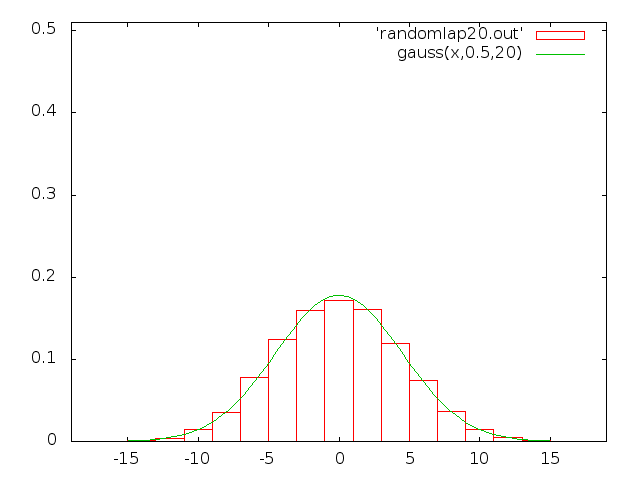
\includegraphics[width=.6\textwidth]{fig/randomlap20}
\caption{Discrete distribution and continuous distribution for set of particles
         in 1D Brownian motion at $t = 20$.}
\label{fig:distr}
\end{figure}
%
This distribution can be seen as the limiting case, with the number of particles
that goes to infinity, while the lenght of the step and the time go to zero, of
the discrete distribution of a randomly walking set of particles, under the
hypothesis that the probability of moving to left or to the right are exactly
$\frac{1}{2}$ each. The distribution, along with the fundamental solution is
plotted in Fig. \ref{fig:distr}.


\section*{Exercise}

Starting from the solution of a previous exercise session on iterative methods
to compute a zero of a function

\begin{enumerate}

  \item Templetize the methods so that they can be used with different 
  floating point number formats.
  
  \item Implement a template functor that manages the function and optionally
  the derivative of the function to be used by the method. Analyze all the
  possible implementation strategy with their advantages and drawbacks. Take
  care in converting also the \cpp{apply} method to a template one.

%  \item () Add a template parameter to the whole class hierarchy. The template is
%  introduced to allow the use of a function or a functor. Also in this case the
%  implementation details can vary, with advantages and drawbacks.

  \item (optional) Substitute the dynamic polymorphism paradigm with a static polymorphism
  paradigm.
\begin{lstlisting}
// dynamic polymorphism
class Base
{
  virtual void foo() {}
};

class Derived: public Base
{
  void foo() {}
};

// static polymorphism
template <typename DerivedT>
class Base
{
  void foo() { static_cast<DerivedT *>(this)->foo(); }
}

class Derived: public Base<Derived>
{
  void foo() {}
};

\end{lstlisting}

\end{enumerate}



\section*{Solution}

\begin{enumerate}

\item Main aspects of the solution for question 1:

\begin{itemize}

\item Both declarations and definitions of templated classes and methods mus be in a header files, for this reason we collected all the class declarations and implementations in one single header file. Other code organizations are possible as explained in the lectures.

\item In a class template derived names are 
resolved only when a template class is instantiated 
so methods and attributes in the derived classes {\tt Bisection}, {\tt Newton}, and {\tt Robust} that are inherited from the base class {\tt IterativeMethod}
must be prepended by {\tt this->} so that the compiler
can understand they are dependent identifiers and only try to resolve them when the templated classes are instantiated.

\item For a similar reason the typedefs in the base
class need to be fully qualified when used in the derived classes.

\item Using the {\tt STL} class template {\tt numeric\_limits}.

\end{itemize}

Main file:

\lstinputlisting{ex8_sol1/bn.cpp}

Header defining all the class templates:
\lstinputlisting{ex8_sol1/iterativeMethod.hpp}

\item Main aspects of the solution for question 2:

\begin{itemize}
\item Notice that, unless specifying {\tt -std=c++11}, a space is required when two {\tt >} 
symbols appear consecutively in a template parameter list.
\end{itemize}

Main file:

\lstinputlisting{ex8_sol2/bn.cpp}

Header defining all the class templates:
\lstinputlisting{ex8_sol2/iterativeMethod.hpp}

\end{enumerate}






\end{document}
